% Desarrollo

This chapter describes the process of design, implementation and configuration of the modular charging station and drone instrumentation. It details the methodologies and tools used to carry out the development, with a focus on creating an effective solution for the charging system.
\section{Charging Station Design and Development}

\subsection{Requirements}
    The following are the technical specifications and requirements for the charging station, ensuring compatibility and efficiency for a drone swarm charging system:     
       \begin{enumerate}
            \item The system shall have a design that is modular and stackable for integration of multiple charging stations. 
            \item The system shall take into account and adapt to the dimensions of the drone proposed for the application.
            \item The system shall have an automatic opening and closing mechanism for the storage drawer of the drone.
            \item The system shall have a charging mechanism for the drone battery.
            \item The system shall contain vision positioning method for the drone.
        \end{enumerate}

\subsection{Materials List}
The following is the materials list used for the construction of the modular charging station. It should be noted that the design and development of this project were largely based on previously available resources and materials, which allowed cost optimization and efficient use of existing inputs.    \begin{itemize}
        \item Aluminum Profiles
            \begin{itemize}
                \item \textbf{30 mm:}
                \begin{itemize}
                \item 4 x Profiles de 100 mm
                \item 4 x Profiles de 810 mm
                \item 6 x Profiles de 750 mm
                \end{itemize}
                \item \textbf{40 mm:}
                \begin{itemize}
                \item 2 x Profiles de 1040 mm
                \item 4 x Profiles de 560 mm
                \item 4 x Profiles de 830 mm
                \item 4 x Profiles de 1120 mm
                \end{itemize}
            \end{itemize}
            \item 16 x 3D printed aluminum profile frames
            \item Aluminum profile turning machine
            \item 2 x Telescopic Correction Riel
            \item 1 x 12V motor
            \item 1 x 3D printed motor brackets
            \item 1 x A V-Belts 1 m 
            \item 2 x Pole type A with internal diameter of 1/2”
            \item 2 x DI Bearing: 15 mm y DE: 35 mm
            \item 2 x 3D printed bearings
            \item 2 x 9 mm MDF 75x75 cm
            \item 8 x 3D printed MDF dividers
            \item 1 x 12V power supply
            \item 1 x Arduino Mega
            \item 1 x Raspberry Pi 4
            \item 1 x H Bridge BTS7960 
            \item 2 x Inductive Proximity Sensor
            \item 1 x Joystick
            \item 1 x WiFi Router
            \item 1 x BT3 Pro Compact Charger
            \item 1 X Cable Carrier 1 m
    \end{itemize}

\subsection{CAD Design of the Charging Base}

To meet the requirements of modular / stackable design and compatibility with the drone in question to the dimensions of the drone. The following CAD design was carried out:
As shown in \ref{fig:etiqueta1} The base known as the “inner drawer” was designed to serve as a platform for takeoff and landing of the drone. This design was made considering the dimensions of the drone and ensuring the inclusion of adequate tolerances to prevent possible collisions. A 30 mm aluminum profile was used in this design, taking advantage of the fact that this material was already available. Other profiles were also integrated in the middle of the box and horizontally, which would support the rails.           
 \begin{figure}[htpb]
                \centering
                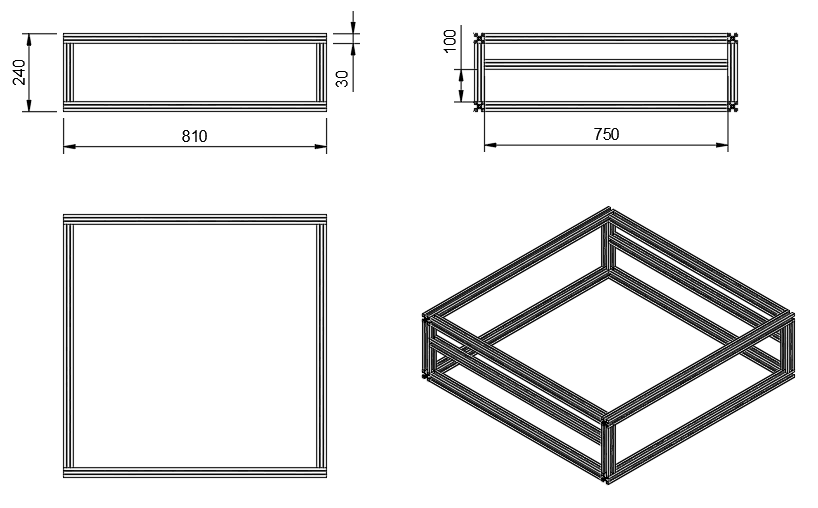
\includegraphics[width=0.8\textwidth]{pictures/PLANOS_CAJON_INTERNO_1.png}
                \caption{Drawing of the internal drawer of the Charging Station}
                \label{fig:etiqueta1}
            \end{figure}
            
            Therefore, taking into account the dimensions of the previous plan, the “external drawer” was made, which is used to store the drone and the electronics of the charging station. This can be seen in \ref{fig:etiqueta2}.           
            \begin{figure}[htpb]
                \centering
                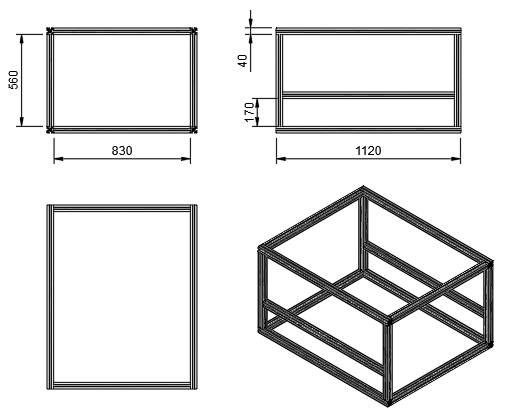
\includegraphics[width=0.8\textwidth]{pictures/PLANOS_CAJON_EXTERNO_1.png}
                \caption{Drawing of the external drawer of the Charging Station}
                \label{fig:etiqueta2}
            \end{figure}

            Then, the dimensions of the landing gear (drone legs) were taken into account to make some mechanical guides (\ref{fig:etiqueta3}) that help them to make a correct magnetic connection with the charging system.            \begin{figure}[htpb]
                \centering
                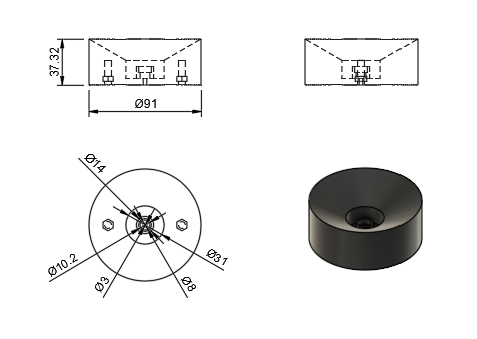
\includegraphics[width=0.8\textwidth]{pictures/PLANO_GUIAS_MECANICAS.png}
                \caption{Mechanical Guidance Drawing for Charging Station}
                \label{fig:etiqueta3}
            \end{figure}


            The necessary CAD designs were developed as shown in \ref{fig:imagen1} and \ref{fig:imagen2} to ensure the correct integration and adaptation of the different components of the charging station. These designs made it possible to establish the essential dimensions, tolerances and features so that each element would fit precisely, ensuring that the charging station would fulfill its functionality efficiently and reliably.The necessary CAD designs were developed as shown in Fig 4. and Fig 5. to ensure the correct integration and adaptation of the different components of the charging station. These designs made it possible to establish the essential dimensions, tolerances and features so that each element would fit precisely, ensuring that the charging station would fulfill its functionality efficiently and reliably.
    \begin{figure}[h]
        \centering
        \begin{minipage}{0.45\textwidth}
            \centering
            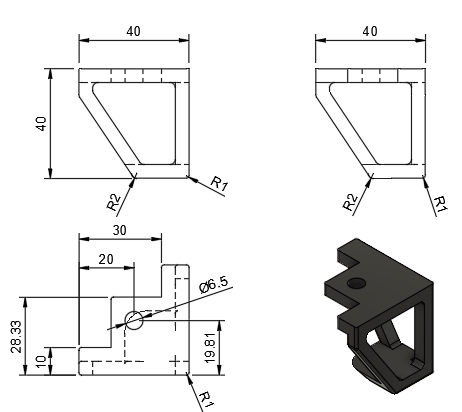
\includegraphics[width=\textwidth]{pictures/PLANO_PATAS_ESTABILIDAD_CAJON.png}
            \caption{Mechanical guide designed to ensure correct positioning of the drone, allowing the drone legs to be magnetically connected to the power supply system.}
            \label{fig:imagen1}
        \end{minipage}%
        \hfill
        \begin{minipage}{0.45\textwidth}
            \centering
            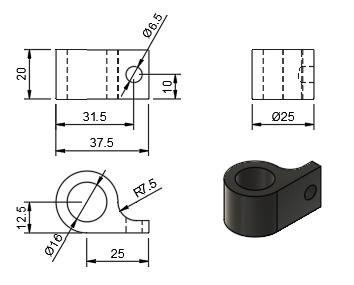
\includegraphics[width=\textwidth]{pictures/PLANO_SENSOR.png}
            \caption{Image 2}
            \label{fig:imagen2}
        \end{minipage}%
        \hfill
    \end{figure}

\subsection{Selection and Implementation of Drawer Motion Mechanism}

Section 2.2.3 explains in detail the different motion mechanisms that were considered for the loading station, evaluating their advantages and disadvantages in terms of accuracy, durability, cost, and ease of integration into the modular design. Options such as linear pistons, toothed belts and other transmission systems were analyzed in order to select a solution that would meet the functionality requirements without increasing costs too much. Tras esta evaluación, se optó por un mecanismo de Polea y Banda tipo V, el cual, además de ser una opción económica, utiliza componentes ya disponibles, como el motor. Este sistema permite un movimiento horizontal suficiente para posicionar el dron con la precisión necesaria para el proceso de carga, a la vez que facilita el apilamiento modular de la estación. La orientación del movimiento no obstruye la estructura general de la estación, lo cual asegura que el diseño cumpla con el requisito de apilabilidad y compatibilidad en espacios compartidos, manteniéndose compacto y adaptable sin comprometer la estructura modular de la estación.

For this mechanism, different components were selected, including a high-strength belt, pulleys, and a DC motor with torque of 0.082 Nm. The belt should support the expected loads, the pulleys (with low friction) would optimize the movement and reduce the wear of the system in continuous operations, and the motor would pull the 3 kg weight of the drone plus the weight of the drawer.
    \subsubsection{CAD Designs y Components}
        \begin{enumerate}
            \item 12V motor
            \item Pole
            \item Band
            \item Baleros
            \item Bearings 
            \item Motor support
        \end{enumerate}

    \subsubsection{V-type Belt and Pulley Mechanism}
    (Mechanism Image)

    \subsection{CAD Design of the Charging Base}
    To meet the requirements of modular / stackable design and compatibility with the drone in question to the dimensions of the drone. The following CAD design was carried out:

        \begin{itemize}
            \item     The design of the main structure of the charging station was made in Fusion 360, considering the minimum dimensions required for the drone and the charging mechanism.
            Image
            \item     The necessary dimension was taken into account so that the drone has a space of at least 10 cm of separation with the wall of the box. This is to avoid any collusion of the drone with the structure of the cargo base when trying to land, also the height of the box was decreased so that the drone can land without problems. On the other hand, we used rails that were obtained previously reused, so the physical charging station is out of the charging base by about 5 cm at the time of being closed. However, in the CAD design, the design is completely closed. 
            Image
            \item     A space of 25 cm was added to place the electronic part of the drawer.
            image
        \end{itemize}



\subsection{Manufacturing Process of the Base Load Frame}

    \begin{enumerate}
        \item \textbf{Material Cutting:}  To start the manufacturing process, precise cuts of the aluminum profiles and MDF boards were made according to the dimensions specified in the materials list. This step is critical to ensure that all parts are assembled correctly in the modular design.
            \begin{center}
                \textit{Image of the cutting process of aluminum and MDF profiles}
            \end{center}
        \item \textbf{Structure Assembly:} Once the parts were cut, the main structure of the loading station was assembled using bolts and nuts to fix the aluminum profiles and the MDF plates using the printed spacers. All parts were checked to ensure that they were aligned and leveled to guarantee the stability and strength of the loading base.
        \begin{center}
                \textit{Image of the assembly process of the load-bearing base structure}
            \end{center}
        \item \textbf{Installation of the Motion Mechanism:} After the main structure was assembled, the V-type pulley and belt mechanism was installed to allow horizontal movement of the caisson. The pulleys, belt, and motor were placed in the previously defined locations, ensuring that the motion system would function properly and without obstructions.
        \begin{center}
                \textit{Image of the installation process of the movement mechanism}
            \end{center}
        
    \end{enumerate}


%%ANABI starts

    \subsection{Electronic Circuit of the Charging Station}

    \subsubsection{Conection Diagram}
    add diagram circuit
    
    \subsubsection{Circuit Construction}
    add images
    
    \subsubsection{Circuit Programming}
    
    \paragraph{\textbf{General Description:}}
    
    
    The described circuit uses a joystick to control a motor that moves a drawer back and forth. The joystick is connected to a microcontroller (Arduino Mega 2560), which reads the joystick's Y-axis values to determine the direction in which the motor should move. Depending on the position of the joystick, the motor moves forward, backward or stops. In addition, limit switches are used to ensure that the motor stops when the drawer reaches its extreme positions.
    
    
    
    \paragraph{\textbf{Main Components}
    }
    \begin{itemize}
        \item \textbf{Arduino:} Microcontroller that manages the reading of the joystick values and controls the motor.
        \item \textbf{Joystick:} Analog input device that allows the user to control the direction of movement.
        \item \textbf{Motor and H-Bridge:} Driver system that moves the drawer. The H-bridge allows controlling the direction and speed of motion of the motor.
        \item \textbf{Limit Switches:} Sensors that detect when the drawer has reached its extreme positions (forward and reverse).
        \item \textbf{Power Supply:} Supplies power to the motor. The Arduino and RaspberryPi4 are supplied power by a plug-in charger.
    \end{itemize}
    
    
    \paragraph{\textbf{Arduino Code}
    }
    
    The Arduino code performs the following functions:
    
    \begin{enumerate}
        \item \textbf{Pin initialization:}
        \begin{itemize}
            \item The joystick pins (A1 for the Y-axis) are configured as inputs.
            \item Motor pins 9 and 8 are configured as outputs.
            \item The limit switch pins (10 and 11) are configured as inputs with internal pull-up resistors.
        \end{itemize}
        \item \textbf{Reading of Joystick:}
        \begin{itemize}
            \item At each loop cycle, the Arduino reads the analog value from the joystick's Y-axis.
            \item Depending on the value read, the Arduino decides whether the motor should move forward, backward or stop.
        \end{itemize}
        \item \textbf{Motor Control:}
        \begin{itemize}
            \item If the value of the joystick Y-axis is greater than 512 (middle position) and the forward limit switch is not pressed, the motor moves forward.
            \item If the Y-axis value is less than 512 and the backward limit switch is not pressed, the motor moves backward.
            \item If the Y-axis value is approximately 512 or any limit switch is pressed, the motor stops.
        \end{itemize}
        \item \textbf{Limit Switch Verification:}
        \begin{itemize}
            \item If the motor is moving forward and the forward limit detects  metal (the drawer), the motor stops.
            \item If the motor is moving backward and the backward limit switch detects  metal (the drawer), the motor stops.
    
        \end{itemize}
        
    \end{enumerate}
    
    %%%%%CODIGOOOOOOOO (??????)
    
    \paragraph{\textbf{Circuit Operation}
    }
    \begin{itemize}
        \item Initialization: At startup, the Arduino configures the pins and establishes serial communication for debugging.
    \item Continuous Readout: In the main loop, the Arduino continuously reads the value of the joystick Y-axis.
    \item Dynamic Control: Based on the value read, the Arduino controls the motor to move the drawer forward, backward or stop it.
    \item Safety Check: Limit switches ensure that the motor automatically stops when the drawer reaches its extreme positions, protecting the system from possible damage.
    \item Debugging: Joystick values and motor status are printed on the serial monitor for easy debugging and system tuning.
    \end{itemize}
    
    \paragraph{\textbf{Annex}
    }
    \paragraph{
    The complete source code for both the Arduino and Raspberry Pi 4 is included in the appendices of this document, making it easy to review and modify as needed for implementation and control of the system.
    
    This approach ensures that the drawer moves in a precise and controlled manner based on the joystick position, providing an efficient solution for linear motion control using a motor and belt.}
    
%%ANABI ENDS
    


\section{Instrumentación del Dron}

\subsection{Especificaciones y Requerimientos}
Para garantizar la compatibilidad y funcionalidad en el sistema de carga, el dron debe cumplir con las siguientes especificaciones:
    \begin{itemize}
        \item Las dimensiones de las piezas deberán adaptarse al frame del drone cuadricoptero de arquitectura abierta que fue comprado.
        \item El dron deberá tener un circuito de carga compatible con la estacion de carga.
        \item El drone deberá contar con una cámara y un sistema de visión para la detección de marcadores Aruco.
        \item Se deberán integrar sensores de localización para la navegación en exterior.
        \item Se deberá integrar algún microprocesador como computadora auxiliar para el procesamiento de datos y la comunicación con la estación de carga.
    \end{itemize}

\subsection{Lista de Materiales para la Instrumentación del Dron} 
    \begin{itemize} 
        \item 1 x Frame de cuadricóptero abierto (especificar modelo) 
        \item 1 x Controlador de vuelo (especificar modelo) 
        \item 1 x Cámara (compatible con detección Aruco) 
        \item 1 x Raspberry Pi 4 (Companion Computer) 
        \item 1 x Sensor de proximidad (modelo de preferencia) 
        \item 1 x Módulo GPS (compatible con el controlador de vuelo) 
        \item Cableado y conectores 
        \item Material de montaje impreso en 3D (soportes específicos para cada componente) 
    \end{itemize}

\subsection{Diseños CAD del Dron} 
Se presentan a continuación los diseños CAD de las piezas que se han desarrollado para el dron, adaptadas a su frame original para integrar los componentes electrónicos necesarios y cumplir con los requisitos de carga y posicionamiento.

    \begin{itemize} 
        \item Se diseñaron nuevos soportes para el microprocesador y la cámara, asegurando una integración estable y precisa en el frame. 
        \item Se implementó un espacio de montaje para los sensores de localización y el circuito de carga. 
        \begin{center} 
            \textit{Imagen de los diseños CAD del dron con las piezas modificadas} 
        \end{center} 
    \end{itemize}

    \subsection{Circuito de Distribución de Energía} 
    El circuito de distribución de energía fue diseñado para proporcionar una alimentación segura y estable a los componentes críticos del dron, incluyendo los motores, el controlador de vuelo, la Raspberry Pi y la cámara. A continuación, se describe el funcionamiento de cada sección del circuito:
    
    \begin{enumerate}
        \item \textbf{Batería LiPo 3S:} 
        Se seleccionó una batería de litio-polímero (LiPo) de 3 celdas con una capacidad de 5200 mAh, un voltaje nominal de 11.1 V y una tasa de descarga de 50C. Esta batería es ideal para proporcionar la corriente necesaria para los motores y los componentes electrónicos sin comprometer la duración de vuelo.
    
        \item \textbf{Distribución de energía a los motores:} 
        La energía de la batería se distribuye a través de una placa de distribución de energía, que conecta la batería a los cuatro controladores electrónicos de velocidad (ESC). Cada ESC regula la energía enviada a su respectivo motor A2212 10T, permitiendo un control preciso de la velocidad de los motores.
    
        \item \textbf{Regulador de voltaje XL4005 DC-DC:} 
        Este regulador convierte el voltaje de 11.1 V de la batería a 5 V, proporcionando una alimentación estable y segura para la Raspberry Pi y la cámara conectada.
    
        \item \textbf{Controlador de vuelo Pixhawk 6X RT:} 
        El controlador de vuelo está conectado directamente a la placa de distribución de energía para recibir la alimentación necesaria. Además, gestiona la comunicación con los ESC y otros sensores del dron, como el módulo GPS (M9N) conectado al puerto GPS1.
    
        \item \textbf{Raspberry Pi 5:} 
        La Raspberry Pi está alimentada a través del regulador de voltaje y se conecta al controlador de vuelo mediante un puerto serial para recibir datos y enviar comandos al sistema. Además, gestiona la cámara conectada por USB, que captura imágenes para el procesamiento en tiempo real.
    
        \item \textbf{Módulo GPS M9N:} 
        Este módulo se conecta al controlador Pixhawk a través del puerto GPS1 para proporcionar datos de posicionamiento en tiempo real en exterior, esenciales para la navegación del dron.
    
    \end{enumerate}
    
    \begin{center}
        \begin{figure}[h!]
            \centering
            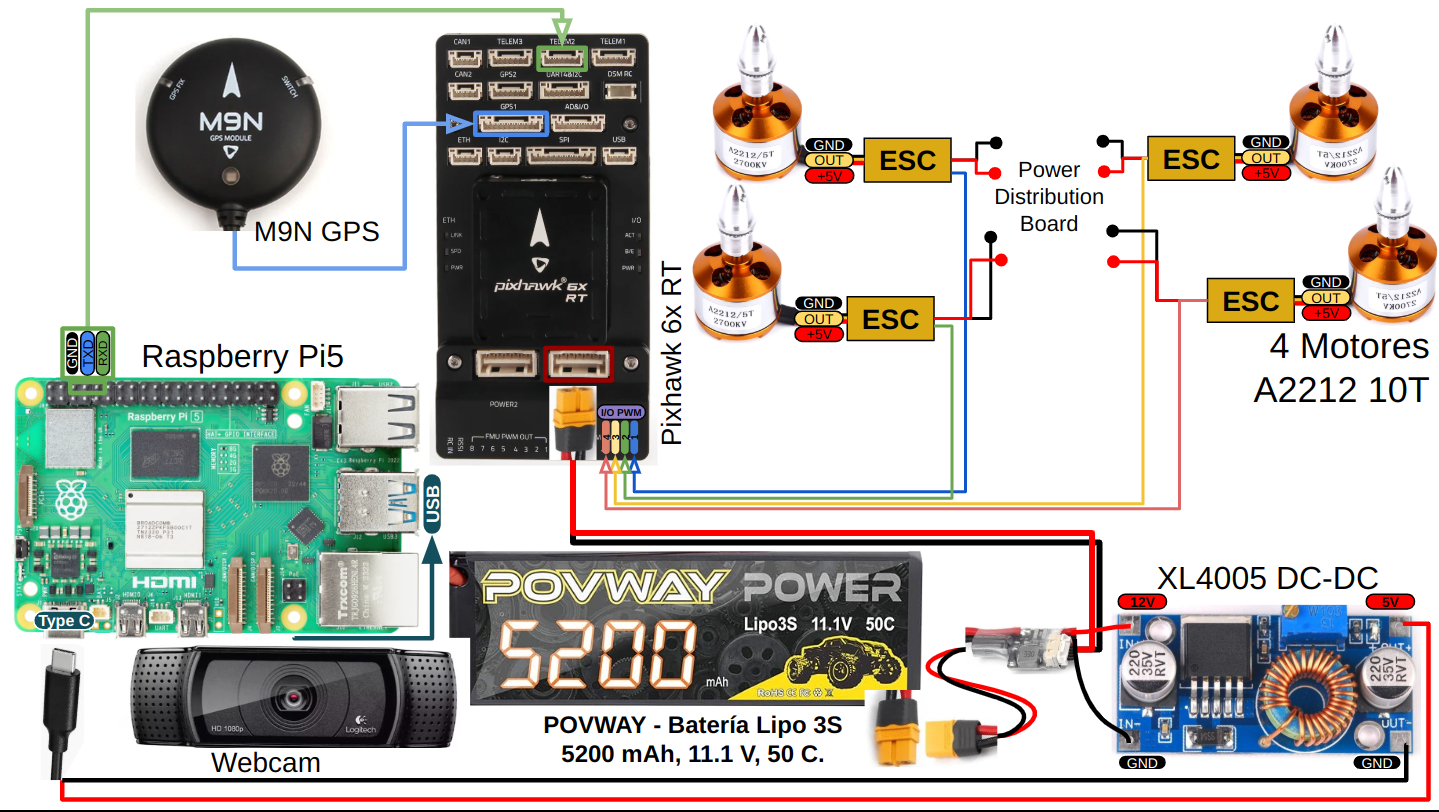
\includegraphics[width=0.8\textwidth]{pictures/drone_electronic_diagram.png}
            \caption{Diagrama del circuito de distribución de energía del dron.}
        \end{figure}
    \end{center}
        

\section{Software Configuration}

\subsection{Configuración de la Computadora Central en Tierra} 
La computadora central se configuró para supervisar y procesar la información proveniente de la computadora auxiliar del dron. A continuación, se describen los pasos realizados para esta configuración:

\begin{itemize}
    \item \textbf{Instalación de ROS 2 Humble:} 
    Dado que la computadora central utiliza Ubuntu 22.04, se instaló ROS 2 Humble siguiendo las instrucciones oficiales. Los comandos utilizados fueron:
    \begin{verbatim}
    sudo apt update && sudo apt install -y software-properties-common
    sudo add-apt-repository universe
    sudo apt update
    sudo apt install -y ros-humble-desktop
    \end{verbatim}
    Esto incluyó la instalación de las herramientas necesarias para desarrollar y ejecutar aplicaciones en ROS 2 Humble.

    \item \textbf{Configuración del entorno:} 
    Para facilitar el uso de ROS 2, se configuró el archivo \texttt{~/.bashrc}. Se agregó la siguiente línea al final del archivo:
    \begin{verbatim}
    source /opt/ros/humble/setup.bash
    \end{verbatim}
    Posteriormente, se ejecutó:
    \begin{verbatim}
    source ~/.bashrc
    \end{verbatim}

    \item \textbf{Clonación del repositorio de GitHub:} 
    Se creó un espacio de trabajo para ROS 2 y se clonó el repositorio correspondiente. Los pasos realizados fueron:
    \begin{verbatim}
    mkdir -p ~/ros2_ws/src
    cd ~/ros2_ws/src
    git clone <URL_del_repositorio>
    cd ..
    colcon build
    \end{verbatim}

    \item \textbf{Configuración del \texttt{ROS\_DOMAIN\_ID}:} 
    Para garantizar una correcta comunicación entre la computadora central y la computadora auxiliar del dron, se configuró el \texttt{ROS\_DOMAIN\_ID} con el valor 10. Esto se realizó añadiendo la siguiente línea al archivo \texttt{~/.bashrc}:
    \begin{verbatim}
    export ROS_DOMAIN_ID=10
    \end{verbatim}
    Luego, se ejecutó:
    \begin{verbatim}
    source ~/.bashrc
    \end{verbatim}
    
    \item \textbf{Verificación del entorno de ROS 2:} 
    Finalmente, se verificó que el entorno estuviera correctamente configurado utilizando los siguientes comandos:
    \begin{verbatim}
    ros2 doctor
    \end{verbatim}
    Esto permitió confirmar que todas las dependencias necesarias para ROS 2 Humble estuvieran instaladas y funcionando correctamente.
    
    \begin{center} 
        \textit{Imagen de la configuración del entorno en la computadora central.} 
    \end{center}
\end{itemize}


\subsection{Configuración de la Computadora Auxiliar del Dron} 
    La Raspberry Pi 5 se configuró como computadora auxiliar para el procesamiento de datos y comunicación en tiempo real con la estación de carga. A continuación, se detallan los pasos realizados para su configuración:
    
    \begin{itemize}
        \item \textbf{Instalación de Ubuntu 24.04:} 
        Se utilizó la herramienta Raspberry Pi Imager para instalar Ubuntu Server 24.04 LTS (64-Bit) en la tarjeta SD. Durante la configuración inicial, se habilitó SSH, se definió un usuario con contraseña y se conectó la Raspberry Pi a la red WiFi.
    
        \item \textbf{Conexión inicial y SSH:} 
        Después de insertar la tarjeta SD en la Raspberry Pi y conectarla a un monitor y teclado, se encendió el dispositivo e ingresaron las credenciales configuradas. Se obtuvo la dirección IP mediante el comando:
        \begin{verbatim}
        hostname -I
        \end{verbatim}
        Con esta información, se estableció una conexión SSH desde una computadora externa utilizando:
        \begin{verbatim}
        ssh <usuario>@<IP>
        \end{verbatim}
        Esto permitió continuar con la configuración de la Raspberry Pi de forma remota.
    
        \item \textbf{Actualización del sistema:} 
        Se realizó una actualización completa del sistema operativo con los siguientes comandos:
        \begin{verbatim}
        sudo apt update && sudo apt upgrade -y
        \end{verbatim}
        También se instaló \texttt{raspi-config} para habilitar el puerto serial. Esta opción se configuró en \texttt{Interface Options > Serial Port}, seleccionando \texttt{No} y luego \texttt{Yes}.
    
        \item \textbf{Modificación de \texttt{bashrc} y configuración del ID:} 
        Para garantizar la comunicación entre todos los dispositivos, se configuró el \texttt{ROS\_DOMAIN\_ID} con el valor 10. Se editó el archivo \texttt{~/.bashrc} con:
        \begin{verbatim}
        sudo vim ~/.bashrc
        \end{verbatim}
        Al final del archivo, se agregaron las siguientes líneas:
        \begin{verbatim}
        export ROS_DOMAIN_ID=10
        source /opt/ros/jazzy/setup.bash
        \end{verbatim}
        Posteriormente, se guardaron los cambios y se ejecutó:
        \begin{verbatim}
        source ~/.bashrc
        \end{verbatim}
    
        \item \textbf{Instalación de ROS 2 Jazzy:} 
        Se siguieron las instrucciones oficiales para instalar ROS 2 Jazzy en Ubuntu 24.04. Esto incluyó los comandos:
        \begin{verbatim}
        sudo apt install -y software-properties-common
        sudo add-apt-repository universe
        sudo apt update
        sudo apt install -y ros-jazzy-desktop
        \end{verbatim}
    
        \item \textbf{Clonación del repositorio de GitHub:} 
        Se creó un espacio de trabajo en ROS 2 para integrar los nodos personalizados. Los pasos realizados fueron:
        \begin{verbatim}
        mkdir -p ~/ros2_ws/src
        cd ~/ros2_ws/src
        git clone <URL_del_repositorio>
        cd ..
        colcon build
        \end{verbatim}
    
        \item \textbf{Instalación de MAVROS y MAVProxy:} 
        Para la comunicación con el Pixhawk, se instalaron MAVROS y MAVProxy. Los comandos utilizados fueron:
        \begin{verbatim}
        sudo apt install ros-jazzy-mavros ros-jazzy-mavros-extras
        sudo rosdep init
        rosdep update
        sudo apt install python3-mavproxy
        \end{verbatim}
        Además, se configuraron los complementos geográficos necesarios:
        \begin{verbatim}
        sudo apt install geographiclib-tools
        sudo geographiclib-get-geoids egm96-5
        \end{verbatim}
    
        \item \textbf{Verificación de la comunicación:} 
        Para garantizar que MAVROS y MAVProxy funcionaran correctamente, primero se inició MAVProxy con:
        \begin{verbatim}
        mavproxy.py --master=/dev/ttyAMA0 --baudrate 921600
        \end{verbatim}
        Posteriormente, se lanzó MAVROS utilizando:
        \begin{verbatim}
        ros2 launch mavros px4.launch fcu_url:=serial:///dev/ttyAMA0:921600
        \end{verbatim}
        Finalmente, se verificaron los tópicos disponibles con:
        \begin{verbatim}
        ros2 topic list
        \end{verbatim}
        y se confirmó la comunicación observando los mensajes de los tópicos relevantes.
        
        \begin{center} 
            \textit{Imagen de la configuración del entorno en la Raspberry Pi 5.} 
        \end{center}
    \end{itemize}
    
\subsection{Configuración de la Estación de Control en Tierra} 
    Se detalla la configuración realizada para la estación de control en tierra utilizando las herramientas QGroundControl y Mission Planner. Ambas aplicaciones son similares en funcionalidad, permitiendo la visualización y gestión de parámetros de vuelo. Sin embargo, dado que se utilizó ArduPilot como firmware, se decidió priorizar Mission Planner debido a su optimización para este sistema.
    
    \begin{itemize}
        \item \textbf{Instalación de Mission Planner y QGroundControl:} 
        Se instalaron ambas herramientas en la computadora central para la gestión y monitoreo del Pixhawk. Mission Planner se utilizó principalmente por su compatibilidad directa con ArduPilot, mientras que QGroundControl fue útil en ciertas configuraciones iniciales como algunas calibraciones redundates.
    
        \item \textbf{Calibración de sensores:} 
        La calibración de los sensores del Pixhawk que se realizó desde Mission Planner, siguiendo estos pasos:
        \begin{itemize}
            \item Acceder a la sección de calibración en la pestaña \textit{Initial Setup}.
            \item Seleccionar la opción de calibración para cada sensor:
            \begin{itemize}
                \item \textbf{Acelerómetro:} Se colocó el Pixhawk en diferentes orientaciones según las instrucciones en pantalla para calibrar correctamente.
                \item \textbf{Giroscopio:} Se mantuvo el Pixhawk inmóvil durante el proceso de calibración.
                \item \textbf{GPS:} Se verificó la recepción de satélites y se ajustaron los parámetros necesarios para una correcta ubicación.
            \end{itemize}
        \end{itemize}
        \begin{figure}
            \centering
            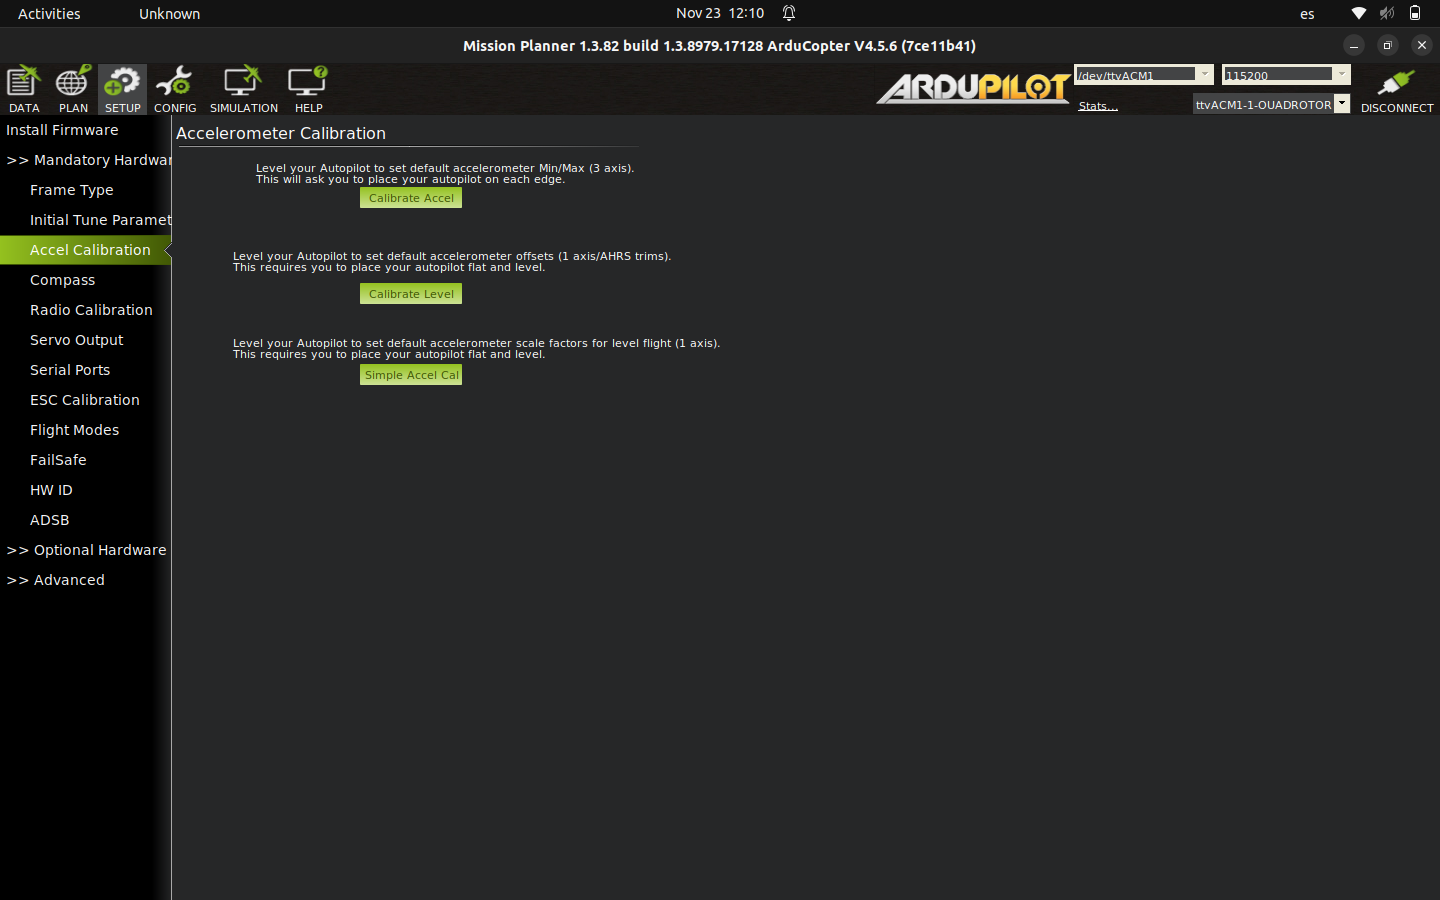
\includegraphics[width=0.8\textwidth]{pictures/mp_calibration.png}
            \caption{Imagen de la configuración de sensores en Mission Planner.}
        \end{figure}

        
        \item \textbf{Parámetros de comunicación:} 
        Para establecer la comunicación entre la Raspberry Pi y el Pixhawk a través de MAVROS y MAVLink, se realizaron los siguientes ajustes en los parámetros utilizando Mission Planner:
        \begin{itemize}
            \item \texttt{SERIAL2\_PROTOCOL}: Configurado en 2 para habilitar MAVLink.
            \item \texttt{SERIAL2\_BAUD}: Ajustado a 921600 para coincidir con la configuración de la Raspberry Pi.
            \item \texttt{SYS\_ID}: Configurado en el ID correspondiente para garantizar una comunicación adecuada con el sistema.
        \end{itemize}
    
    \end{itemize}
    

\section{Sistema de Visión}
\subsection{Especificaciones y Requerimientos} 
El sistema de visión debe cumplir con los siguientes requisitos para garantizar la detección precisa de marcadores Aruco:
    \begin{itemize}
        \item Obtener las matrices de calibración intrínsecas y extrínsecas de la cámara.
        \item Generar y detectar marcadores Aruco de distintos tamaños en tiempo real.
    \end{itemize}

\subsection{Calibración de la Cámara} 
El proceso de calibración de la cámara se realizó utilizando un script en Python con la biblioteca OpenCV. Este procedimiento se detalla a continuación, combinando fragmentos del código y las imágenes obtenidas en cada etapa. El código completo se encuentra en los anexos del documento.
    
    \begin{enumerate}
        \item \textbf{Captura de imágenes:} 
        Se recopilaron múltiples imágenes del tablero de ajedrez desde diferentes ángulos y distancias para abarcar todo el campo de visión de la cámara. Estas imágenes presentaban distorsiones propias de la lente, como se observa en la Figura \ref{fig:imagen_descalibrada}.

        \begin{center}
            \begin{figure}[h!]
                \centering
                %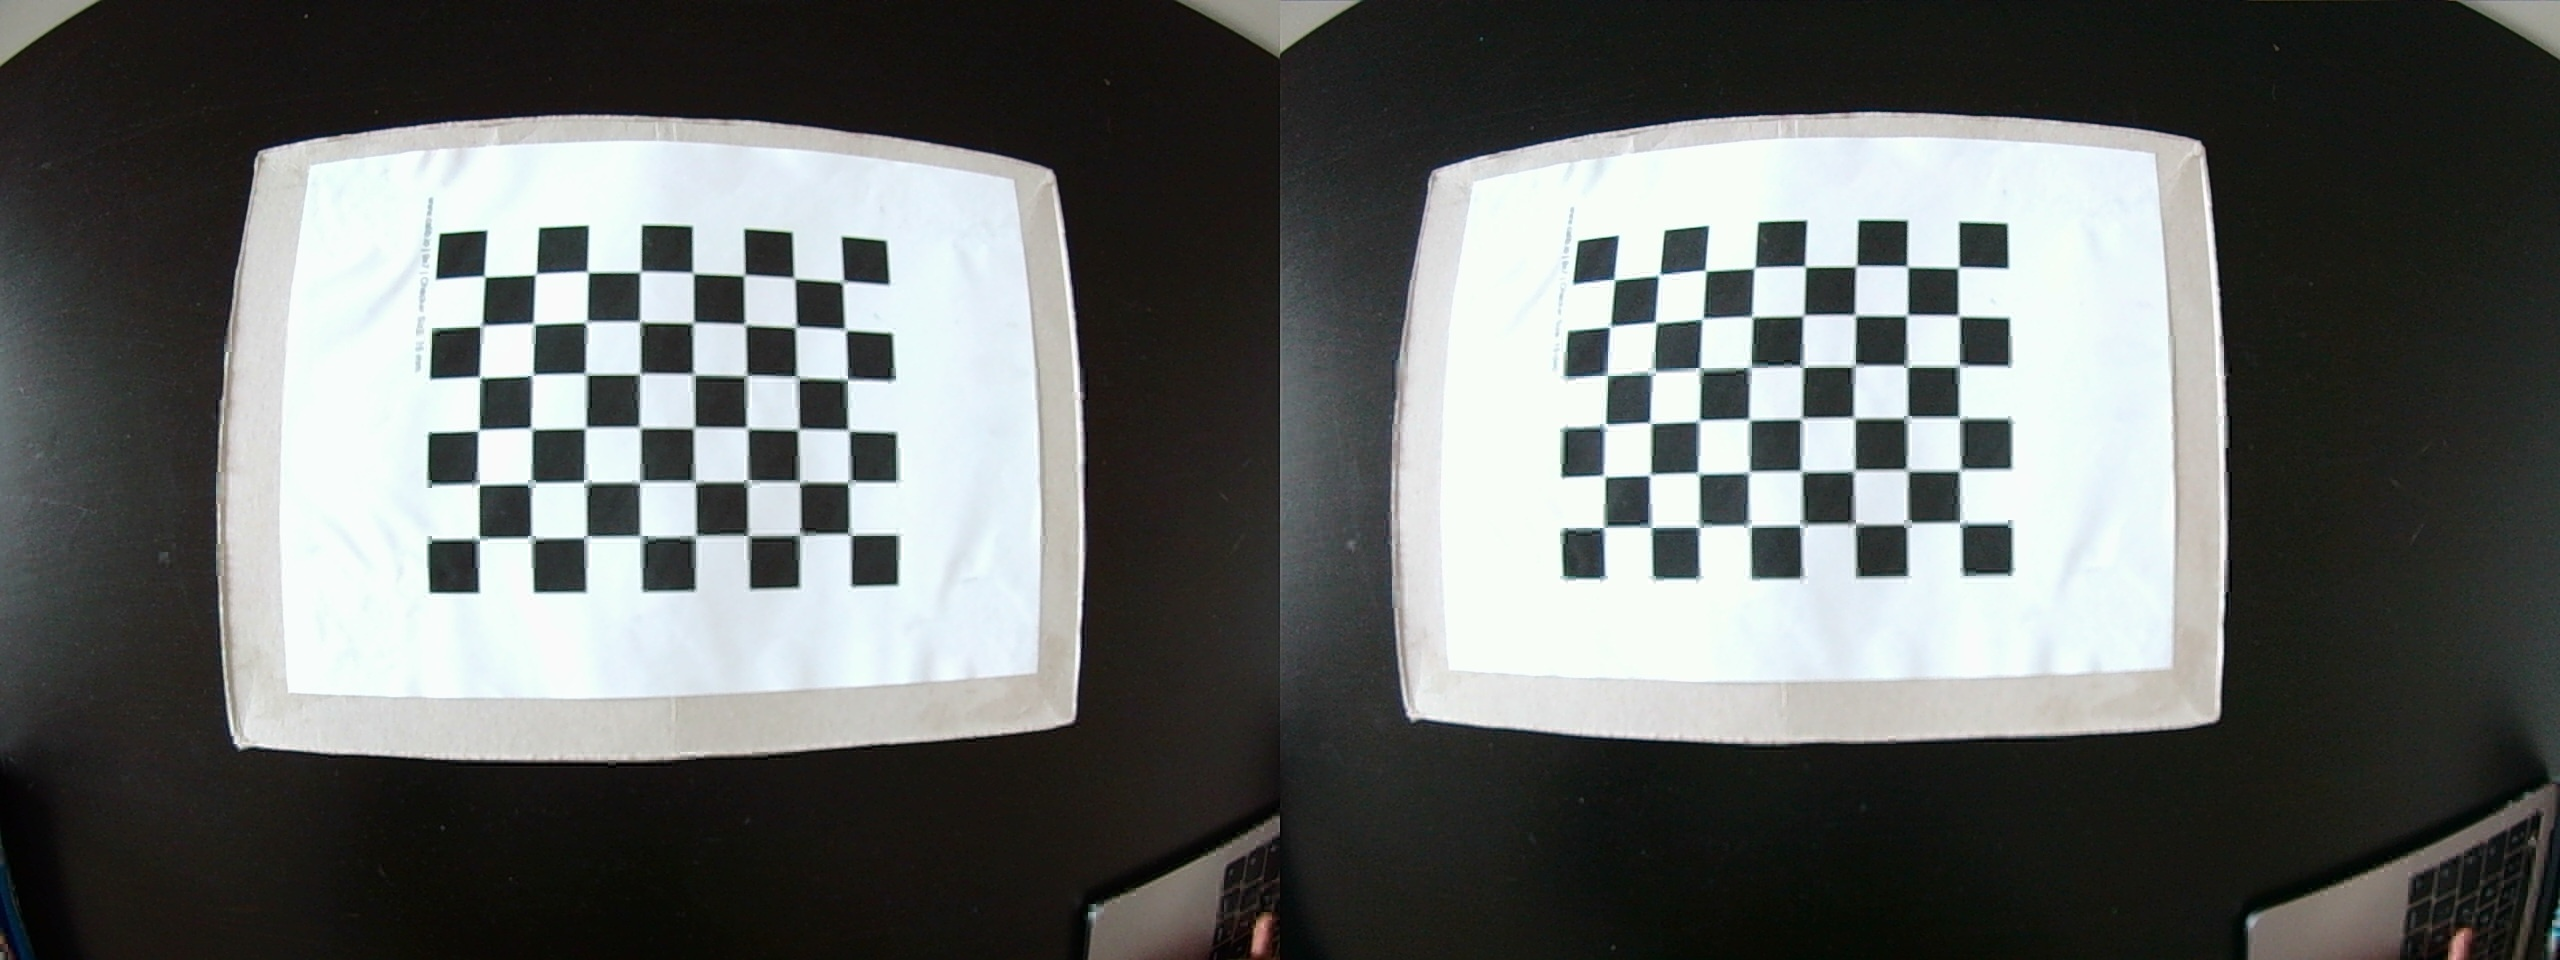
\includegraphics[width=0.8\textwidth]{pictures/imagen_descalibrada.png}
                \caption{Ejemplo de imagen descalibrada tomada durante el proceso de captura.}
                \label{fig:imagen_descalibrada}
            \end{figure}
        \end{center}
    
        \item \textbf{Detección de esquinas:} 
        El script detectó las esquinas internas del tablero de ajedrez mediante la función \texttt{cv2.findChessboardCorners}. Posteriormente, se refinaron las esquinas detectadas utilizando \texttt{cv2.cornerSubPix}, y se visualizaron las líneas superpuestas en las imágenes de calibración, como se muestra en la Figura \ref{fig:det_ejemplos}.
        \begin{verbatim}
        ret, corners = cv2.findChessboardCorners(gray, (ncols, nrows), None)
        corners2 = cv2.cornerSubPix(gray, corners, (11, 11), (-1, -1), criteria)
        \end{verbatim}
        \begin{center}
            \begin{figure}[h!]
                \centering
                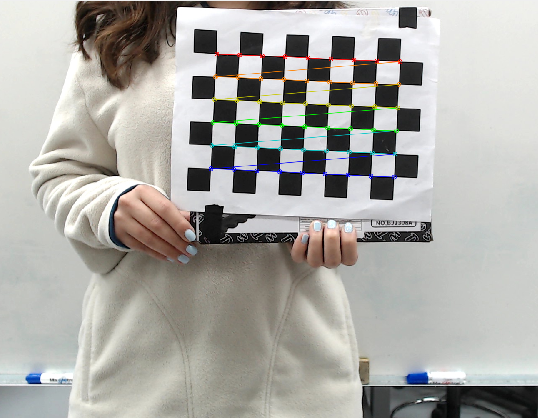
\includegraphics[width=0.8\textwidth]{pictures/calib_predictions.png}
                \caption{Detección y refinamiento de esquinas en el tablero de ajedrez.}
                \label{fig:det_ejemplos}
            \end{figure}
        \end{center}
    
        \item \textbf{Calibración de la cámara:} 
        Utilizando \texttt{cv2.calibrateCamera}, se calcularon los parámetros intrínsecos de la cámara y los coeficientes de distorsión. Estos parámetros permiten corregir las distorsiones en las imágenes capturadas. La Figura \ref{fig:imagen_calibrada} muestra el resultado después de aplicar estos parámetros.
        \begin{verbatim}
        ret, mtx, dist, rvecs, tvecs = cv2.calibrateCamera(objpoints, 
                                                           imgpoints, 
                                                           img_size, 
                                                           None, 
                                                           None)
        \end{verbatim}
        Donde:
        \begin{itemize}
            \item \texttt{mtx}: Matriz intrínseca de la cámara.
            \item \texttt{dist}: Coeficientes de distorsión.
            \item \texttt{rvecs}, \texttt{tvecs}: Rotaciones y traslaciones.
        \end{itemize}
        \begin{center}
            \begin{figure}[h!]
                \centering
                %\includegraphics[width=0.8\textwidth]{pictures/imagen_calibrada.png}
                \caption{Imagen calibrada después de aplicar los parámetros obtenidos.}
                \label{fig:imagen_calibrada}
            \end{figure}
        \end{center}
    
        \item \textbf{Cálculo del error de calibración:} 
        Se verificó la precisión del modelo calculando el error promedio mediante \texttt{cv2.projectPoints}. Este cálculo compara las esquinas detectadas y proyectadas.
        \begin{verbatim}
        error = cv2.norm(imgpoints[i], imgpoints2, cv2.NORM_L2) / len(imgpoints2)
        print("Total error: {}".format(mean_error / len(objpoints)))
        \end{verbatim}
    
        \item \textbf{Almacenamiento de parámetros:} 
        Los parámetros de calibración obtenidos se guardaron en un archivo JSON, lo que permite su reutilización en futuros procesos de corrección de imágenes.
        \begin{verbatim}
        data = {"camera_matrix": mtx.tolist(), 
                "distortion_coefficients": dist.tolist()}
        with open(output_path, "w") as file:
            json.dump(data, file, indent=4)
        \end{verbatim}
    \end{enumerate}
    
    
\subsection{Generación de Marcadores ArUco} 
    Se generaron marcadores ArUco adaptados al sistema, incluyendo tamaños y patrones específicos. En particular, se crearon marcadores embebidos, donde un marcador interno se incrusta dentro de un marcador externo para maximizar la precisión en la detección. A continuación, se describe el proceso paso a paso, destacando las partes importantes del código utilizado. El código completo se encuentra en los anexos del documento.
    
    \begin{enumerate}
        \item \textbf{Carga del diccionario de ArUco:} 
        Se utilizó el diccionario predefinido \texttt{DICT\_6X6\_250} de OpenCV, adecuado para generar marcadores con diferentes patrones y niveles de detalle.
        \begin{verbatim}
        aruco_dict = aruco.getPredefinedDictionary(aruco.DICT_6X6_250)
        \end{verbatim}
    
        \item \textbf{Generación del marcador externo:} 
        Se definió un tamaño de 220 píxeles para el marcador externo (\texttt{outer\_marker\_size}) y se generó el marcador con un ID específico (\texttt{outer\_marker\_id}). Esto permitió crear un marcador grande que sirviera como contenedor.
        \begin{verbatim}
        outer_marker = aruco.generateImageMarker(aruco_dict, 
                                                 outer_marker_id, 
                                                 outer_marker_size)
        \end{verbatim}
        \begin{center}
            \begin{figure}[h!]
                \centering
                
\includegraphics[width=0.4\textwidth]{pictures/aruco_marker_5.png}
                \caption{Marcador ArUco externo generado.}
            \end{figure}
        \end{center}
    
        \item \textbf{Generación del marcador interno:} 
        El marcador interno se generó con un tamaño de 50 píxeles (\texttt{inner\_marker\_size}) y un ID específico (\texttt{inner\_marker\_id}). Este marcador se diseñó para ser incrustado dentro del marcador externo.
        \begin{verbatim}
        inner_marker = aruco.generateImageMarker(aruco_dict, 
                                                 inner_marker_id, 
                                                 inner_marker_size)
        \end{verbatim}

        \begin{center}
            \begin{figure}[h!]
                \centering
                
\includegraphics[width=0.2\textwidth]{pictures/aruco_marker_100.png}
                \caption{Marcador interno con borde blanco añadido.}
            \end{figure}
        \end{center}
    
        \item \textbf{Creación del borde blanco alrededor del marcador interno:} 
        Se añadió un borde blanco de un píxel alrededor del marcador interno utilizando \texttt{cv2.copyMakeBorder}, lo que facilita su incrustación y aumenta la visibilidad en diferentes condiciones de iluminación.
        \begin{verbatim}
        inner_marker_with_border = cv2.copyMakeBorder(
            inner_marker,
            top=border_size,
            bottom=border_size,
            left=border_size,
            right=border_size,
            borderType=cv2.BORDER_CONSTANT,
            value=255  # Blanco
        )
        \end{verbatim}
        
    
        \item \textbf{Incrustación del marcador interno en el marcador externo:} 
        Se calculó la posición central para incrustar el marcador interno con borde en el marcador externo. El marcador externo se modificó para incluir un fondo negro en el centro antes de insertar el marcador interno con borde.
        \begin{verbatim}
        center_position = (outer_marker_size - inner_marker_with_border_size) // 2
        e_aruco_marker[center_position:center_position + inner_marker_with_border_size,
                       center_position:center_position + inner_marker_with_border_size] = 0
        e_aruco_marker[center_position:center_position + inner_marker_with_border_size,
                       center_position:center_position + inner_marker_with_border_size] = inner_marker_with_border
        \end{verbatim}
        \begin{center}
            \begin{figure}[h!]
                \centering
                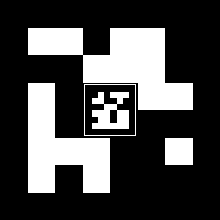
\includegraphics[width=0.4\textwidth]{pictures/embedded_aruco.png}
                \caption{Marcador ArUco embebido generado.}
            \end{figure}
        \end{center}
    
        \item \textbf{Almacenamiento del marcador embebido:} 
        Finalmente, el marcador generado se guardó como una imagen PNG para su uso posterior.
        \begin{verbatim}
        cv2.imwrite(f'embedded_aruco_marker_{outer_marker_id}_{inner_marker_id}.png', 
                    e_aruco_marker)
        \end{verbatim}
    \end{enumerate}


\subsection{Detección de Marcadores e-Aruco en Tiempo Real} 
    El sistema fue diseñado para detectar marcadores Aruco en tiempo real, utilizando imágenes capturadas por una cámara conectada al dron. Este proceso se llevó a cabo mediante un nodo en ROS2 que procesa las imágenes y estima la pose de los marcadores con respecto a la cámara. El código completo se encuentra en los anexos del documento. A continuación, se describe el paso a paso del sistema:
    
    \begin{enumerate}
        \item \textbf{Publicación de imágenes desde el dron:} 
        La computadora auxiliar en el dron (companion computer) publica imágenes comprimidas capturadas por la cámara a un tópico de ROS 2 (\texttt{/camera\_image/compressed}). Estas imágenes se envían a la computadora en tierra para su procesamiento.
    
        \item \textbf{Recepción de imágenes en la computadora en tierra:} 
        Un nodo en la computadora en tierra se suscribe a las imágenes publicadas por el dron y realiza las siguientes tareas:
        \begin{itemize}
            \item Convierte las imágenes comprimidas en matrices utilizables para el procesamiento con OpenCV.
            \item Redimensiona las imágenes y las convierte a escala de grises para optimizar la detección.
        \end{itemize}
    
        \item \textbf{Detección de marcadores Aruco:} 
        Se utiliza la biblioteca OpenCV para detectar los marcadores Aruco presentes en la imagen. Los pasos incluyen:
        \begin{itemize}
            \item Uso del diccionario \texttt{DICT\_6X6\_250} para identificar marcadores específicos.
            \item Cálculo de las esquinas de los marcadores detectados mediante \texttt{aruco.detectMarkers}.
            \item Dibujo de los marcadores detectados para su visualización.
        \end{itemize}
        \begin{center}
            \begin{figure}[h!]
                \centering
                %\includegraphics[width=0.8\textwidth]{pictures/deteccion_arucos.png}
                \caption{Detección de marcadores Aruco en la imagen procesada.}
            \end{figure}
        \end{center}
    
        \item \textbf{Estimación de la pose:} 
        Para cada marcador detectado, se calculó su posición y orientación en el espacio con respecto a la cámara. Esto se realizó utilizando la función \texttt{aruco.estimatePoseSingleMarkers}, que devuelve:
        \begin{itemize}
            \item \texttt{tvec}: Vector de traslación (\textit{x}, \textit{y}, \textit{z}) en metros.
            \item \texttt{rvec}: Vector de rotación que se convierte en ángulos de Euler (\textit{roll}, \textit{pitch}, \textit{yaw}) mediante matrices de rotación.
        \end{itemize}
        \begin{center}
            \begin{figure}[h!]
                \centering
                %\includegraphics[width=0.8\textwidth]{pictures/calculo_pose.png}
                \caption{Representación gráfica de la posición y orientación calculada de un marcador Aruco.}
            \end{figure}
        \end{center}
    
        \item \textbf{Visualización y publicación de resultados:} 
        Los resultados obtenidos, incluyendo la pose de los marcadores, se visualizaron en tiempo real y se publicaron en un nuevo tópico de ROS 2 (\texttt{/aruco\_detection/compressed}). Las imágenes procesadas contenían:
        \begin{itemize}
            \item Marcadores detectados con esquinas resaltadas.
            \item Ejes X, Y y Z proyectados para mostrar la orientación de cada marcador.
        \end{itemize}
        \begin{center}
            \begin{figure}[h!]
                \centering
                %\includegraphics[width=0.8\textwidth]{pictures/marcadores_ejes.png}
                \caption{Imagen con marcadores detectados y ejes proyectados.}
            \end{figure}
        \end{center}
    
        \item \textbf{Correcciones de posición:} 
        Basándose en los valores de \texttt{tvec}, se calcularon las correcciones necesarias para ajustar la posición del dron con respecto al marcador, incluyendo movimientos laterales (\textit{x}), verticales (\textit{y}) y de profundidad (\textit{z}).
    
        \item \textbf{Interacción con el sistema:} 
        Los resultados de la detección de marcadores Aruco se utilizaron para visualizar la posición y orientación del drone en tiempo real, lo que permitirá posteriormente que el sistema de control pueda ajustar las mismas para su aterrizaje en la estación de carga.
    \end{enumerate}
    

\section{Sistema de Comunicación}

    \subsection{Especificaciones y Requerimientos} 
    El sistema de comunicación entre el dron y la estación de carga fue diseñado para garantizar la transferencia eficiente y en tiempo real de datos críticos. Los requisitos principales son:
    
    \begin{itemize}
        \item \textbf{Red local basada en WiFi:} 
        Proporcionar una comunicación efectiva entre los dispositivos sin necesidad de acceso a Internet.
        \item \textbf{Middleware DDS de ROS 2:} 
        Utilizar la arquitectura de nodos y tópicos de ROS 2 para gestionar la comunicación de datos entre los dispositivos conectados.
    \end{itemize}
    
    \subsection{Estructura de Comunicación} 
    
    \subsubsection{Red Local WiFi} 
    La red local fue creada utilizando un router WiFi que conecta todos los dispositivos involucrados en el sistema, incluyendo el dron, la estación de carga y la computadora en tierra. Esta configuración eliminó la necesidad de Internet, proporcionando un entorno seguro y aislado para la transmisión de datos. El dron, equipado con una computadora auxiliar, transmitió datos mediante tópicos de ROS 2, como imágenes comprimidas y mensajes de estado, hacia la estación de carga y la computadora en tierra.
    
    \begin{figure}
        \centering
        %\includegraphics[width=0.8\textwidth]{pictures/wifi_network.png}
        \caption{Diagrama de la red local WiFi utilizada en el sistema.}
    \end{figure}
    
    \subsubsection{Comunicación mediante ROS 2} 
    El sistema utilizó la arquitectura de nodos y tópicos de ROS 2 para gestionar la comunicación entre los dispositivos. Cada dispositivo en la red cumplió funciones específicas relacionadas con la publicación y suscripción de datos relevantes:
    
    \begin{itemize}
        \item \textbf{Dron:} 
        Publicó imágenes de la cámara (\texttt{/camera\_image/compressed}) y datos de estado relacionados con la batería, posición y otros parámetros críticos.
        \item \textbf{Computadora en tierra:} 
        Contiene una interfaz que se suscribió a los tópicos publicados por el dron para:
        \begin{itemize}
            \item Procesar imágenes y calcular la posición de los marcadores Aruco.
            \item Mostrar datos de estado del dron, como nivel de batería y modo de vuelo, etc. en tiempo real.
            \item Publicar comandos hacia la estación de carga, como abrir o retraer el cajón de la estación, mediante tópicos específicos.
        \end{itemize}
        \item \textbf{Estación de carga:} 
        Se suscribió a los comandos enviados desde la interfaz de la computadora en tierra para ejecutar las acciones necesarias, como la apertura y cierre del cajón.
    \end{itemize}
    
    \begin{figure}
        \centering
        %\includegraphics[width=0.8\textwidth]{pictures/ros2_comms.png}
        \caption{Diagrama de comunicación entre los dispositivos utilizando ROS 2.}
    \end{figure}
    

    




